\documentclass{article}


% if you need to pass options to natbib, use, e.g.:
%     \PassOptionsToPackage{numbers, compress}{natbib}
% before loading neurips_2022


% ready for submission
\usepackage{neurips_2022}


% to compile a preprint version, e.g., for submission to arXiv, add add the
% [preprint] option:
%     \usepackage[preprint]{neurips_2022}


% to compile a camera-ready version, add the [final] option, e.g.:
%     \usepackage[final]{neurips_2022}


% to avoid loading the natbib package, add option nonatbib:
%    \usepackage[nonatbib]{neurips_2022}


\usepackage[utf8]{inputenc} % allow utf-8 input
\usepackage[T1]{fontenc}    % use 8-bit T1 fonts
\usepackage{hyperref}       % hyperlinks
\usepackage{url}            % simple URL typesetting
\usepackage{booktabs}       % professional-quality tables
\usepackage{amsfonts}       % blackboard math symbols
\usepackage{nicefrac}       % compact symbols for 1/2, etc.
\usepackage{microtype}      % microtypography
\usepackage{xcolor}         % colors
\usepackage{amsmath}
\usepackage{graphics} %SHOMIK ADDED THESE
\usepackage{graphicx} %SHOMIK ADDED THESE

\title{Implicit Score Guided Attention for \\ Causal Inference}


% The \author macro works with any number of authors. There are two commands
% used to separate the names and addresses of multiple authors: \And and \AND.
%
% Using \And between authors leaves it to LaTeX to determine where to break the
% lines. Using \AND forces a line break at that point. So, if LaTeX puts 3 of 4
% authors names on the first line, and the last on the second line, try using
% \AND instead of \And before the third author name.


\author{%
  David S.~Hippocampus\thanks{Use footnote for providing further information
    about author (webpage, alternative address)---\emph{not} for acknowledging
    funding agencies.} \\
  Department of Computer Science\\
  Cranberry-Lemon University\\
  Pittsburgh, PA 15213 \\
  \texttt{hippo@cs.cranberry-lemon.edu} \\
  % examples of more authors
  % \And
  % Coauthor \\
  % Affiliation \\
  % Address \\
  % \texttt{email} \\
  % \AND
  % Coauthor \\
  % Affiliation \\
  % Address \\
  % \texttt{email} \\
  % \And
  % Coauthor \\
  % Affiliation \\
  % Address \\
  % \texttt{email} \\
  % \And
  % Coauthor \\
  % Affiliation \\
  % Address \\
  % \texttt{email} \\
}


\begin{document}


\maketitle


 


\section{Research Question}
What's in-between a partially linear and fully non-parametric model?


\section{Two Starting Points}
\begin{enumerate}
    \item Why don't most of the models that we fit in applied economics have a generative modeling component? 
    \item Why do we need to go beyond linear/partially-linear models
    
\subsection{Second Starting Point}
\begin{figure}[htbp]
\centering
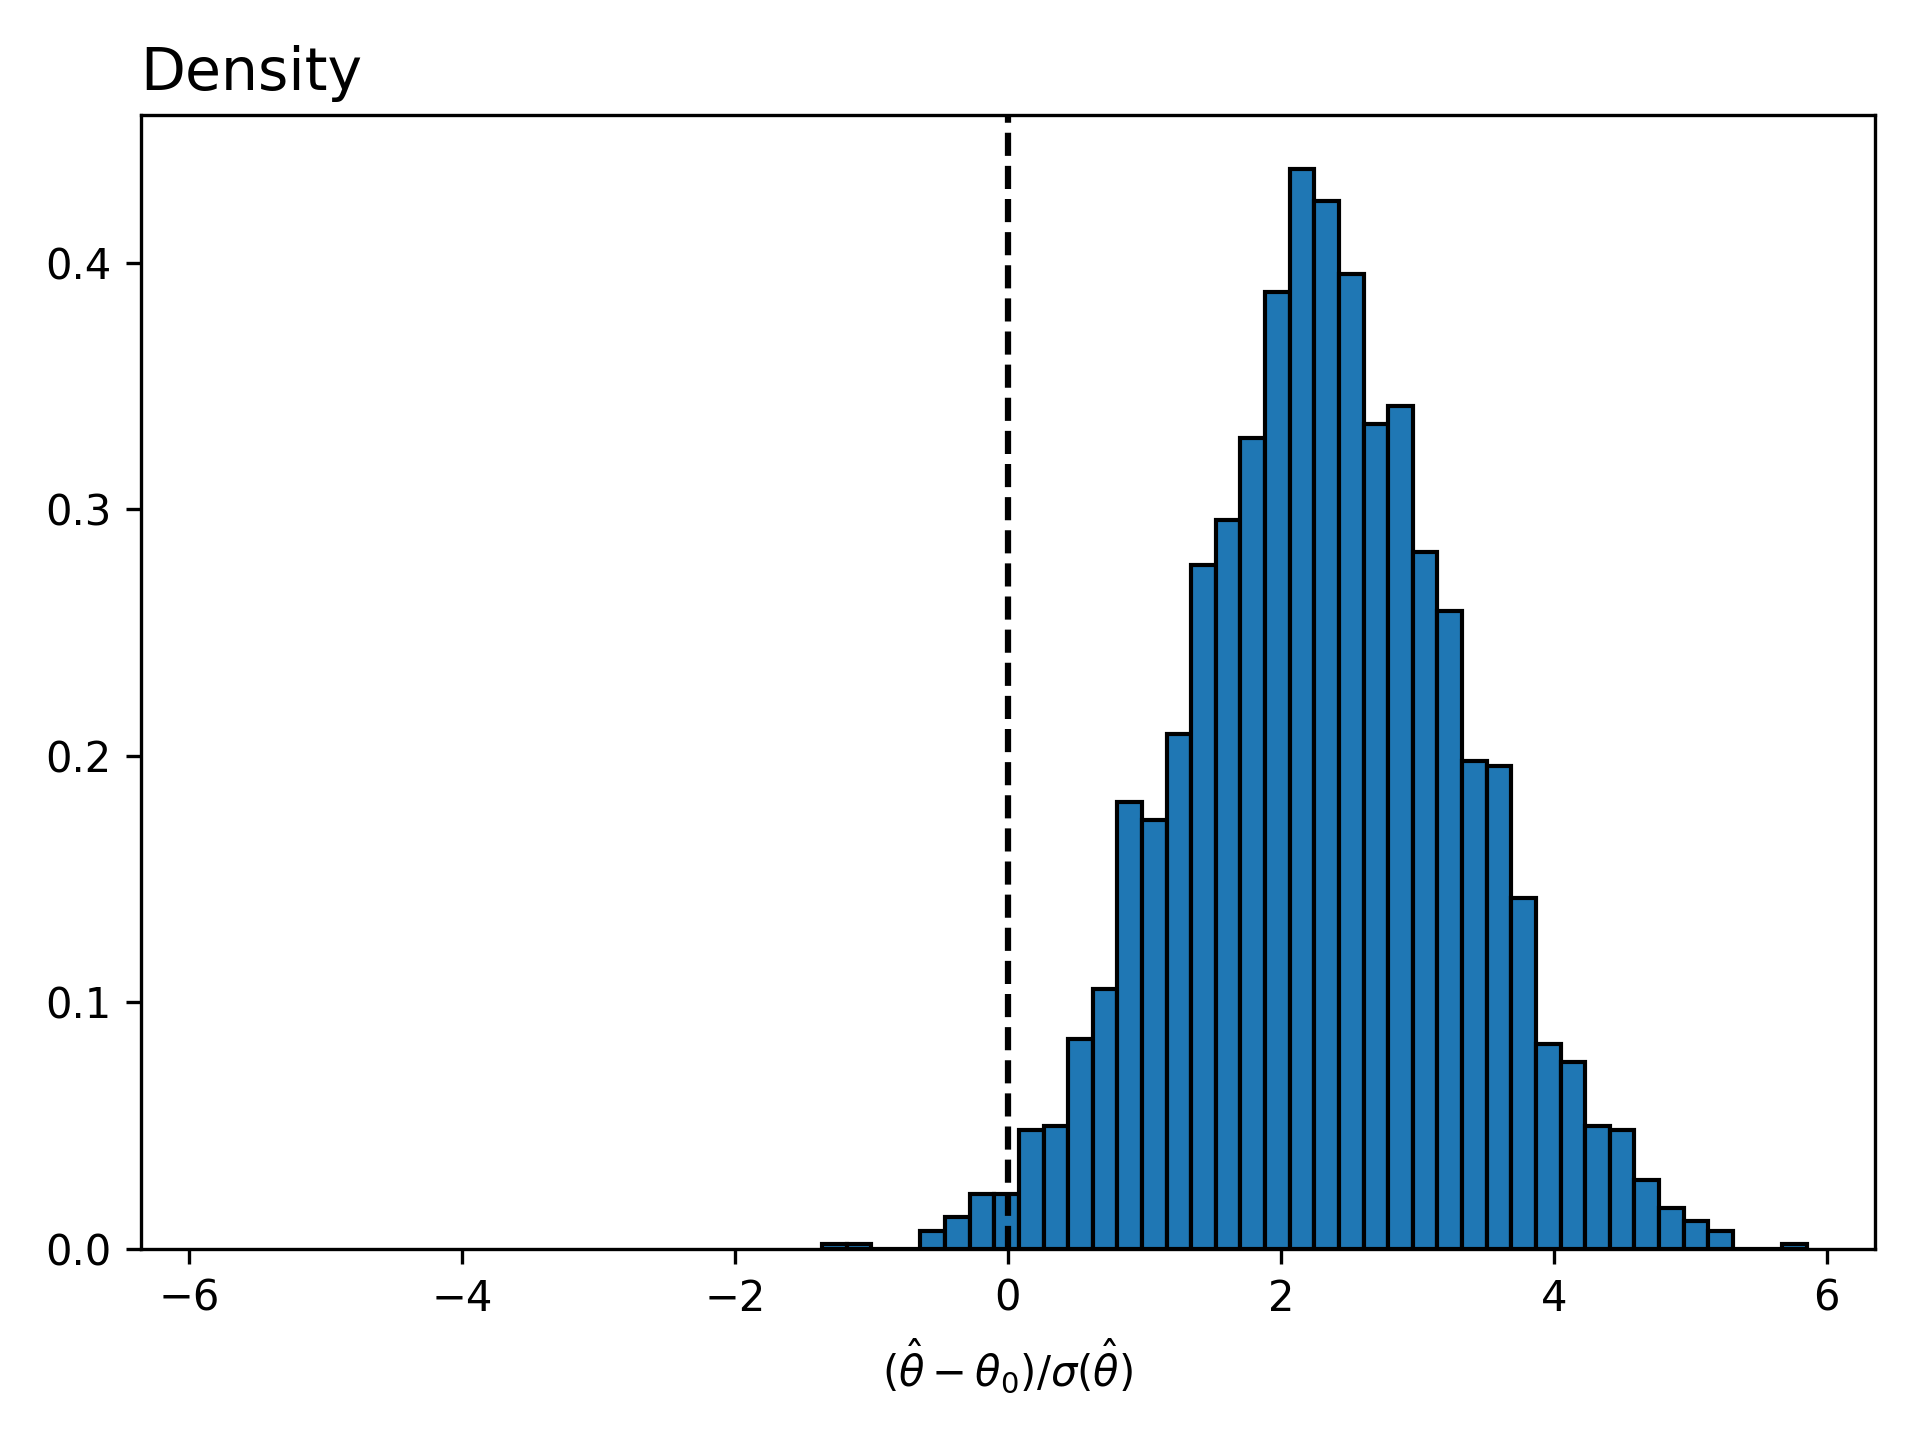
\includegraphics[scale=0.5]{examples/dml.png}
\label{fig:nonparametrics}
\end{figure}
\end{enumerate}


\section{Working Hypothesis}
Maybe we don't need a full generative model.
\section{Theory}
\begin{itemize}
    \item \href{https://arxiv.org/abs/1902.04742}{Uniform convergence may be unable to explain generalization in deep learning
} shows that $\varepsilon _{\text{stat}}$ may be meaninglessly high!\footnote{see this \href{https://youtu.be/plIJYzVKfdI?list=PLn2-dEmQeTfSLXW8yXP4q_Ii58wFdxb3C&t=1961}{lecture}}

\begin{align*}
\varepsilon _{\text{opt}} + \varepsilon _{\text{stat}} + \varepsilon _{\text{appr}}    
\end{align*}
\item Why doesn't the lipschitz condition take into account some aspect of similarity? 
\begin{align*}
    \| f(x) - f(x') \| \leq \beta \| x- x' \| 
\end{align*}
\end{itemize}
\begin{itemize}
    \item With high dimensional data, can you learn an appropriate weighting? If not, why even do a partially linear model?
    \item Is economic data on a low dimensional manifold? 
    \item Is it possible to think of treatment heterogeneity as existing along a low dimensional manifold?
    \item The weighting depends on those around it. 
\end{itemize}
The partially linear model is in some sense the best you can do if you stick to a regression only approach. 
\begin{itemize}
    \item Map neural network into kernel methods 
    \item Suggest correction for kernel methods 
    \item map correction into neural network training
\end{itemize}
\newpage 
\subsection{Diffusion Models}
\subsubsection{Objective}
\begin{align*}
\intertext{Sampling From the Empirical Distribution}
    &\textrm{key} \longmapsto f(\textrm{key}) = \textrm{jax.random.choice(key, X)} \\ 
\intertext{Sampling from a Parameterized Distribution}
    &\textrm{key} \longmapsto f(\textrm{key}) = \textrm{SamplingModel(key, params)}
\end{align*}
\subsubsection{Set-up}
We have class of Gaussian random variables that are parameterized by our training data 
\begin{align*}
\textrm{key} \longmapsto f(\textrm{key}, x_0) = \textrm{ForwardModel(key}, x_0)
\end{align*}
\section{Probability Theory}
 
\begin{itemize}
    \item Probability Space: $\big(\Omega, \mathcal{F}, \mathbb{P}\big)$
    \item Index Set: $T$
    \item State Space: $\big(E, \mathcal{E}\big)$
    \item Stochastic Process: $\{X_t: \Omega \rightarrow E \}_t$
\end{itemize}
\newpage 
\section{Introduction}
Quarterbacks on a freshman team are often taught to look only at one side of the field when considering who to target. As they progress in their development, the begin to consider the entire field, and perhaps get to a level where the head coach is comfortable with them positioning their teamates, and making adjustments to the play based on what they observe pre-snap.\par 

Fitting linear models with an aim towards causal inference can have a bit of a freshman quarterback feel to it. There's this narrow and often singular concern as to whether $x$ is correlated with $\varepsilon$ with  little discussion about optimization, generative modeling, or learning topics of that nature.

\end{document}
